\documentclass[12pt]{article}

\usepackage[utf8]{inputenc}       % .tex-file text encoding
\usepackage[T1]{fontenc}          % vector fonts and special chars in
\usepackage{graphicx} % include external images

\usepackage{natbib}
\setcitestyle{square,comma,numbers, sort&compress}
\bibliographystyle{unsrtnat}
\newcommand{\doi}[1]{\href{http://www.dx.doi.org/#1}{doi:#1}}

\usepackage{booktabs}
\usepackage{amsmath}

\usepackage[a4paper]{geometry}
\geometry{
  top         = 2.54cm,
  bottom      = 2.54cm,
  inner       = 2cm,
  outer       = 2.54cm,
  footskip    = 11mm,
  headheight  = 1cm,
  headsep     = 0.75cm,
  showframe   = false
}

% change spacing
\setlength{\parskip}{0.5ex}
\setlength{\parindent}{0cm}

\graphicspath{ {fig/} }
\hyphenation{}

%--- Meta data ---------------------------------------------------------

\usepackage{hyperref}
\hypersetup{
pdfauthor   ={Jonas Schöley, Ricarda Duerst},
pdftitle    ={},
pdfsubject  ={},
pdfkeywords ={},
hidelinks,
breaklinks=true,
colorlinks=false
}

%--- Titlepage ---------------------------------------------------------

\begin{document}

\begin{titlepage}

  {\textbf{Title:}
  Empirical prediction intervals applied to short term mortality forecasts and excess deaths
  \par\medskip}

  {\textbf{Authors:}
  Jonas Schöley$^{1}$, Ricarda Duerst$^{1}$
  \par\medskip}

  {\textbf{Affiliations:}\par
  $^1$ Max Planck Institute for Demographic Research; Rostock, Germany\par
  \par\medskip}

  {\textbf{Corresponding authors:}\par
  Jonas Schöley \href{mailto:schoeley@demogr.mpg.de}{\texttt{schoeley@demogr.mpg.de}}\par
  \par\medskip}

  %{\textbf{Keywords:}
  %excess deaths; COVID-19; cross-validation; robustness
  %\par\medskip}

  {\textbf{Abstract:}
  We propose empirical prediction intervals for the study of weekly expected and excess deaths and demonstrate the superior coverage and generality of these intervals compared with conventional parametric intervals. Instead on relying on the suitability of parametric assumptions or the magnitude of errors over the fitting period, empirical prediction intervals are estimated from cross-validated time series of past prediction errors, reflecting the intuitive notion that a forecast is only as precise as similar forecasts in the past turned out to be. We further employ empirical prediction intervals to assess the level of excess mortality which can reliably be detected two years into the pandemic, given the error of our methods.
  \par\medskip}

\end{titlepage}

%--- Text --------------------------------------------------------------

\section*{Background}

We propose empirical prediction intervals for the study of weekly expected and excess deaths and demonstrate the superior coverage and generality of these intervals compared with conventional parametric intervals.

Mortality forecasts on a sub-annual timescales have gained relevance as the basis for excess deaths calculations during the COVID-19 pandemic. Framed as a forecasting problem, one aims to predict the weekly deaths which would have happened without COVID-19 by forecasting deaths over the pandemic period based on pre-pandemic trends. Those forecasted ''expected deaths`` are associated with an error which can probabilistically be expressed as a ''prediction interval`` within which the true expected deaths are to be found with a given probability.It is well known that prediction intervals around forecasted values tend to be too narrow. In the context of COVID-19 excess death modeling this phenomenon may lead to wrong conclusions regarding the impact of the pandemic on population mortality, by giving an overly optimistic picture on how precise one can actually measure excess deaths more than two years into the pandemic.

Empirical prediction intervals, instead on relying on correct parametric specifications, estimate the distribution of error around a forecasted value from actual past, out-of-sample forecasting errors. The idea is simple: One quantifies the distribution of error around a forecast by applying the forecasting method to an equivalent forecasting problem where the true value is known. In contrast to the cross-validation method of forecast assessment one seeks to estimate the full distribution of forecast error indexed over all desired forecasting strata and time points. In order to do so, a statistical model is fitted to known out-of-sample forecasting errors.

Research on empirical uncertainty intervals has been ongoing for at least half a century \cite{Williams1971}. The 1980s saw active demographic reasearch on empirical intervals and the authors generally found that the intervals based on past error have better coverage than model based intervals, see e.g. \cite{Stoto1983}, \cite{Cohen1986}, \cite{Smith1988}.

In the machine learning literature there is growing interest in ''distribution free uncertainty quantification``, given that popular techniques do not provide an intrinsic estimate of uncertainty. The community has build a theory on empirical uncertainty intervals under the term ''Conformal prediction``. Here too, the idea is to look at the distribution of historical error measures to assess how likely any given future deviation from the prediction would be.

Interest in empirical prediction intervals saw a recent resurgence in the context of algorithmic prediction methods, for which probabilistic errors are hard or impossible to derive. The community has build a theory on empirical uncertainty intervals under the term ''Conformal prediction``. The idea is to look at the distribution of historical error measures to assess how likely any given future deviation from the prediction would be \cite{Shafer2008}.

We demonstrate the construction and coverage of empirical prediction intervals via the example of weekly death counts in Denmark. The task is to estimate expected weekly death counts and prediction intervals over a period of 2 years starting 2018. We compare the coverage of the empirical prediction intervals with conventional parametric intervals.

\section*{Data and Methods}

Data on weekly deaths was sourced from the Short Term Mortality Fluctuations Database (STMF)\cite{Jdanov2021a}. The data was split into four partially overlapping data series with 7 years of training data followed by a 2 year forecasting horizon each. While the first three data series (Figure \ref{fig:figure-1}A) are used for the estimation of the empirical forecasting error, the fourth series (Figure \ref{fig:figure-1}C) is reserved for the application and validation of the empirical uncertainty interval method -- in an applied scenario, this would be the forecast of interest.

\begin{figure}[ht!]
    \centering
    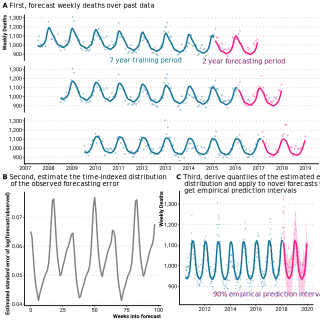
\includegraphics[width=0.9\textwidth]{figure_1.pdf}
     \caption{Empirical prediction intervals are derived from the time-indexed distribution of past forecasting errors. Shown here is the example for expected Danish weekly death counts for the years 2018 to 2020.}
     \label{fig:figure-1}
\end{figure}

First, we modelled the expected deaths at time $t$ (measured in weeks since some origin), $\hat y_t$, as

\begin{equation*}
  \log \hat y_t = \alpha + \beta_tt + s_w(w[t]),
\end{equation*}

where $\beta_tt$ captures a long term trend and $s_w(w[t])$ is a cyclical penalized spline over week-of-year to reflect the seasonality of death counts. The weekly deaths were assumed to be distributed as

\begin{equation*}
  Y_t \sim \mathrm{Neg.Binomial}(\hat y_t, \phi).
\end{equation*}

Parametric prediction intervals for this model were derived via sampling of the posterior predictive distribution.

This model is representative of much of the applied work in excess death modeling, where regression approaches are prominent, but note that any other forecasting algorithm could have been chosen instead to demonstrate the method of empirical prediction intervals. We fitted this model over the 7 years fitting period in each data series and predicted over a two year horizon following the training data (Figure \ref{fig:figure-1}AC).

As a measure of forecasting error we defined $\epsilon_t$ to be the logged ratio between forecasted and observed deaths at time $t$.

\begin{equation*}
\epsilon_t = \log\frac{\hat y_t} {y_t}
\end{equation*}

We modelled this error via a normal distribution with zero mean\footnote{Additionally, we could have modelled the mean error over time in order to estimate and correct for the biases of a forecasting model} and time-varying standard-deviation $\sigma_t$,

\begin{align*}
    \epsilon_t &\sim \mathrm{Normal}(0, \sigma_t) \\
    \log \sigma_t &= \alpha + \beta_tt + s_w(w[t]),
\end{align*}

where $\beta_tt$ captures a linear trend in the variance of the log relative forecasting error over time (i.e. increasing uncertainty over the forecasting horizon), and $s_w(w[t])$ captures the seasonality of the error variance as a function of week-of-year. In the context of expected deaths modeling this seasonality is pronounced due to the challenges in predicting the severity of flu-waves during winter. Other models, such as a non-parametric quantile regression, are possible as well. We fitted this model to the out-of-sample forecasting errors of the first three data series (Figure \ref{fig:figure-1}B).

Once estimates for $\sigma_t$ were found we derived the quantiles around the forecasted expected deaths $\hat y_t$ of the fourth data series with the help of the standard-normal distribution (Figure \ref{fig:figure-1}C):

\begin{equation*}
  Q_p(\hat y_t) = \exp[\log \hat y_t + \sigma_t\Phi^{-1}(p)].
\end{equation*}

\clearpage

\section*{Preliminary Results}

The empirical prediction intervals display a substantially better coverage compared to the parametric intervals, which are too narrow (Table \ref{tab:coverage}). In the final publication we will demonstrate the consequences of these wider prediction intervals for the analysis of excess deaths during the COVID-19 pandemic. Given the empirical error of our methods for calculating expected deaths, which level of excess deaths can we reliably detect two years into the pandemic?

\begin{table}[ht]
  \centering
  \begin{tabular}{
  llll
  }
  \toprule
  & \multicolumn{3}{c}{Nominal coverage} \\
  & 50\% & 90\% & 95\% \\
   \midrule
Actual coverage of & & & \\
Parametric intervals  & 30.6 & 66.3 & 77.6 \\
Empirical  intervals & \bfseries49.0 & \bfseries87.8 & \bfseries90.8 \\
   \bottomrule
\end{tabular}
\caption{Comparing the nominal and actual coverage of parametric vs. empirical prediction intervals over the forecasting period. Note that the coverage of the empirical prediction intervals is evaluated on a separate validation set from the one used to construct the interval.}
\label{tab:coverage}
\end{table}


\clearpage

%--- Bibliography ------------------------------------------------------

\bibliography{epunc.bib}

\clearpage

\end{document}
